\documentclass[epsfig]{article}
\usepackage{epsfig}
\usepackage{amsmath}
\usepackage{graphicx} 
\usepackage{float}
%\usepackage{mfpic}

\textwidth 6.7in
\oddsidemargin -0.1in
\textheight 8.50in
\topmargin -0.55in
\renewcommand{\textfraction}{0.25}
\renewcommand{\floatpagefraction}{0.7}
\markboth{}{\sl E. Mer\'enyi \hfil COMP / ELEC / STAT 502 \hfil Homework 3 }
\pagestyle{myheadings}

\def\bpar{\vskip26pt}
\def\npar{\vskip13pt}
\def\spar{\vskip10pt}

\begin{document}


\parindent=0pt

{\bf 
\npar
Zhuo Chen, Yidan Pan

Equally contributed
\bpar
}
\bpar
\centerline{\bf Homework 3}
\npar
\begin{centering}{Total possible score: 60 points, 60 points = 100\%\\}
\end{centering}
\npar




\bpar
{\bf Problem 1.}
\spar
\begin{figure}[htbp] 
\centering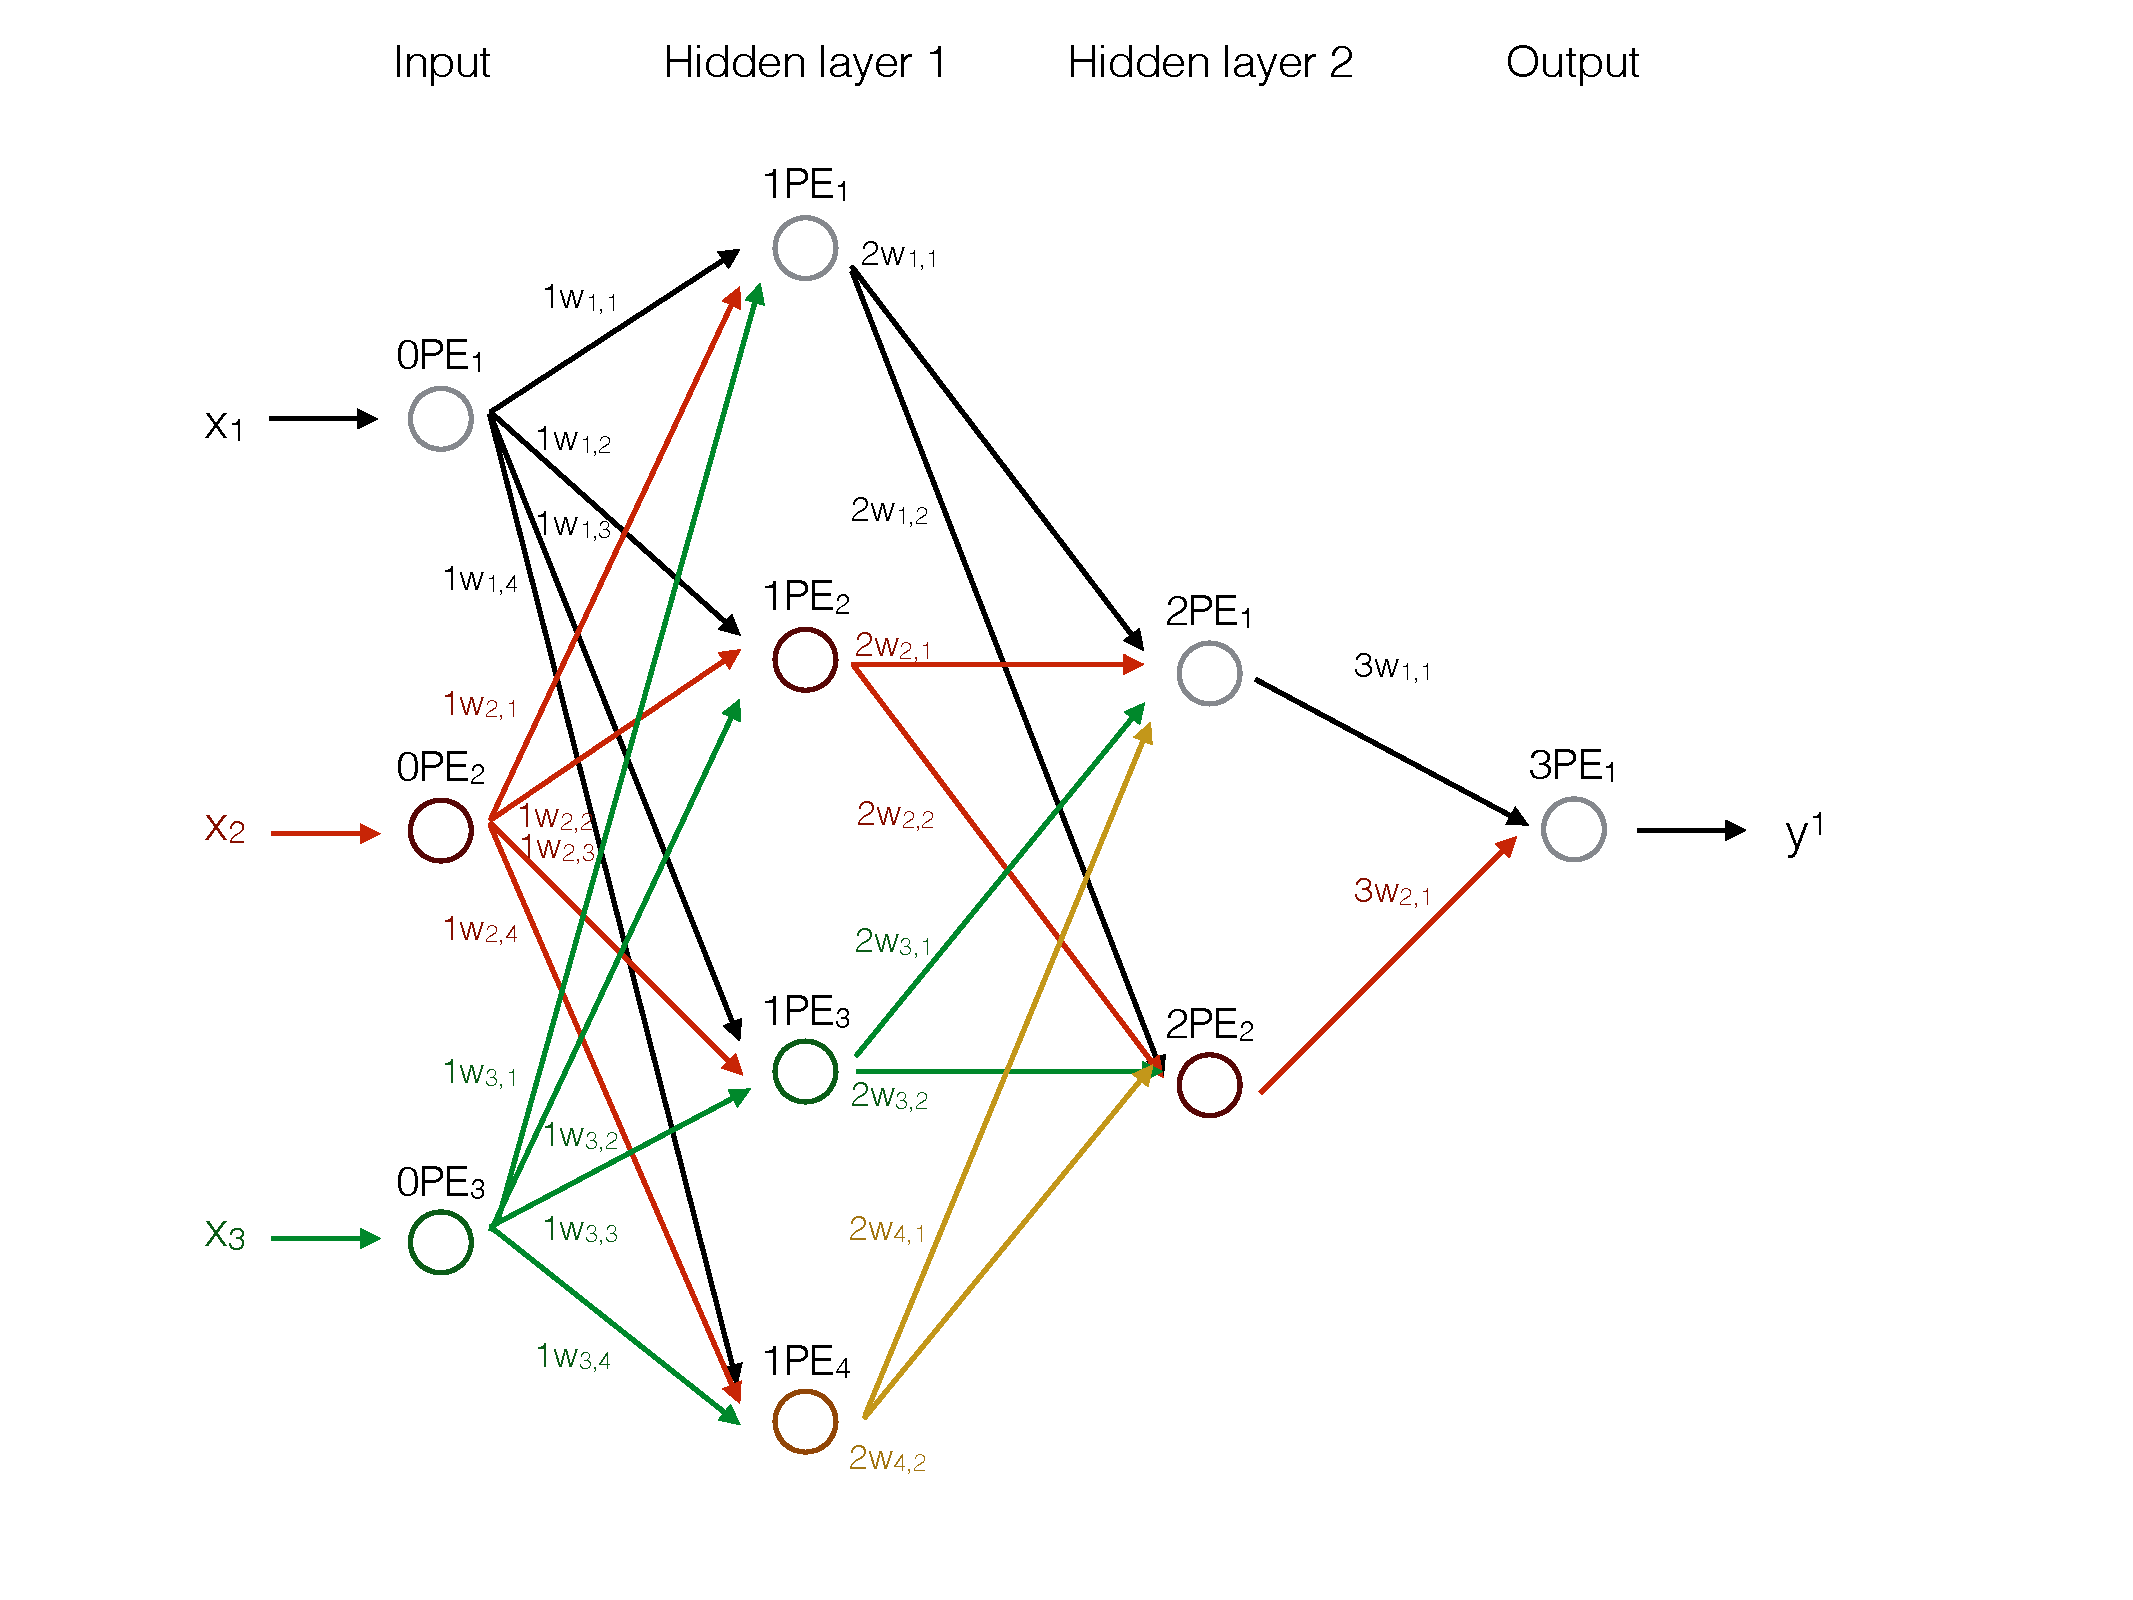
\includegraphics[width=7 in]{Hw3fig1.pdf} 
\end{figure} 

\spar

\bpar
{\bf Problem 2.}

i) 
\spar
Assume that ${\textbf{x}}$ is an nx1 vector:

For the linear transfer in feed forward network ${F:\textbf{x} \rightarrow \textbf{y}}$, we can write it as:

$${F(x_i)=w_{i1}x_1+w_{i2}x_2+\dots +w_{in}x_n}= \textbf{w}_ix_i=y_i$$

where i=1,2,....n

Therefore:

$${\textbf{y}=\{y_1,\dots, y_n\} = \{ \textbf{w}_1x_1,\dots,  \textbf{w}_nx_n\} = \textbf{Wx}}$$

 
\spar

ii) \spar
The structural complexity of linear transfer will not change during transfer and the errors will maintain:
Assume the true input as $\textbf{x}_i$(the ideal input)+$\textbf{x}$(error in input), then:

$${\textbf{y}=\{y_1,\dots, y_n\} = \textbf{W}(\textbf{x}+\textbf{e})=\textbf{Wx}+\textbf{We}}$$

The result of transfer will always be the linear combination of input.



\bpar\npar
{\bf Problem 3.}
\spar
a)\spar
Show the original character images in matlab:
\spar
	\centerline{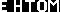
\includegraphics[width=3.5in]{oricha.png}} 
\spar
Then we modified the data by changing 0 to -1 and reshape the matrix. We got a $ 144 \times 5 $ matrix, and it's used as X(input) and Y(desired output). Then we used function errcorr.m to train the network,and got the memory.\\

\begin{figure}[H] 
	\centering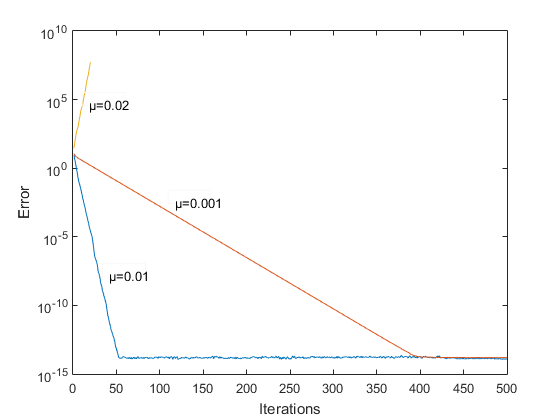
\includegraphics[width=4.5in]{train.png} 
	\caption{Changing of error along with iterations. Here the error is 2-norm(Y-MX)}\label{fig:1} 
\end{figure} 

From fig.1 we can see when $\mu=0.02$ the function cannot converge. For $\mu$=0.01 or 0.001 the function can converge, so we pick $\mu=0.01$ and 
tol=$10^{-5}$, $max n=100$. Also we can see the error could be controled lower then $10^{-13}$, which means the recall error of the training set is very low. Since the matrix can almost perfectly recall the training image, so we didn't show the difference map here.\spar

b)\spar

Flip the image, then recall it with the memory trained in (a). With different corruption fraction we have\\ 
\begin{figure}[H] 
	\centerline{Corrupted input image}
	\centering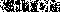
\includegraphics[width=2.5in]{p20.png} 
		\centerline{Recalled image}
		\centering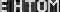
\includegraphics[width=2.5in]{p22.png} 
			\centerline{Difference image}
			\centering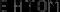
\includegraphics[width=2.5in]{p2d.png}
			 	\centerline{Tresholded recalled image}
						\centering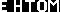
\includegraphics[width=2.5in]{oricha.png} 
	\caption{Recall with 20\% corrupted data.   }\label{fig:1} 
\end{figure} 
\begin{figure}[H] 
	\centerline{Corrupted input image}
	\centering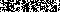
\includegraphics[width=2.5in]{p33i.png} 
	\centerline{Recalled image}
	\centering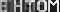
\includegraphics[width=2.5in]{p33.png} 
	\centerline{Difference image}
	\centering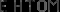
\includegraphics[width=2.5in]{p33d.png}
	\centerline{Tresholded recalled image}
	\centering
\includegraphics[width=2.5in]{p33o.png} 
	\caption{Recall with 30\% corrupted data.   }\label{fig:2} 
\end{figure} 
\begin{figure}[H] 
\centerline{Corrupted input image}
\centering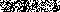
\includegraphics[width=2.5in]{p44i.png} 
\centerline{Recalled image}
\centering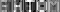
\includegraphics[width=2.5in]{p44.png} 
\centerline{Difference image}
\centering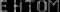
\includegraphics[width=2.5in]{p44d.png}
\centerline{Tresholded recalled image}
\centering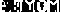
\includegraphics[width=2.5in]{p44o.png} 
\caption{Recall with 40\% corrupted data.   }\label{fig:2} 
\end{figure} 
\begin{figure}[H] 
\centerline{Corrupted input image}
\centering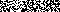
\includegraphics[width=2.5in]{p55i.png} 
\centerline{Recalled image}
\centering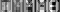
\includegraphics[width=2.5in]{p55.png} 
\centerline{Difference image}
\centering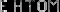
\includegraphics[width=2.5in]{p55d.png}
\centerline{Tresholded recalled image}
\centering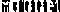
\includegraphics[width=2.5in]{p55o.png} 
\caption{Recall with 50\% corrupted data.   }\label{fig:2} 
\end{figure} 
\begin{center}
	\begin{tabular}{| l | l | l | l | l|}
		\hline
		Corruption Fraction & 0.2 & 0.3 & 0.4 &0.5 \\ \hline
		Error(2-norm(Y-MX)) & 7.5 & 9.7 & 12.8 &15.6 \\ \hline
		Fraction of mismatched pixels& 0\% & 2.7\% & 12.4\% &50.6\%\\ \hline

	\end{tabular}
\end{center}
* All the images is rescaled to [-1,1].\\
** Error is computed by avaraging several different runs.
\spar

c)
\spar
We used 20\% corrupted data for training input and clean data for desired output. The training parameters are same as part (a).
\begin{figure}[H] 
	\centerline{Corrupted input image}
	\centering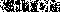
\includegraphics[width=3.5in]{p20.png} 
	\centerline{Desired output image}
	\centering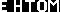
\includegraphics[width=3.5in]{oricha.png} 

\end{figure} 
The training curve is similar to part(a).
\begin{figure}[H] 
	\centering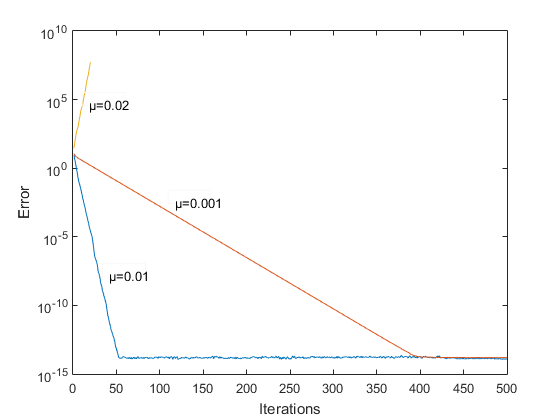
\includegraphics[width=4.5in]{train.png} 

\end{figure} 
Then we test the recall accurancy of different input:
\begin{center}
	\begin{tabular}{| l | l | l | l | l| l|}
		\hline
		Difference fraction to training set & 0.2 & 0.3 & 0.4 &0.5 & clean data*  \\ \hline
		Error(2-norm(Y-MX)) & 6.9 & 9.6 & 13.1 &15.4& 6.4 \\ \hline
		Fraction of mismatched pixels& 0\% & 3.7\% & 11.9\% &51.4\% & 0\%\\ \hline
		
	\end{tabular}
\end{center}
*Clean data also have 20\% different pixels from training data.
\npar
\begin{figure}[H] 
	\centerline{Input image}
	\centering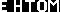
\includegraphics[width=3.5in]{oricha.png} 
	\centerline{Recalled image}
	\centering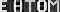
\includegraphics[width=3.5in]{p3d.png} 
	\centerline{Difference image}
	\centering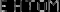
\includegraphics[width=3.5in]{p3e.png}
	\centerline{Tresholded recalled image}
	\centering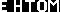
\includegraphics[width=3.5in]{oricha.png} 
	\caption{Recall with clean data.   }\label{fig:1} 
\end{figure} 
\begin{figure}[H] 
	\centerline{Input image}
	\centering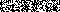
\includegraphics[width=3.5in]{q3i.png} 
	\centerline{Recalled image}
	\centering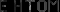
\includegraphics[width=3.5in]{q3d.png} 
	\centerline{Difference image}
	\centering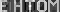
\includegraphics[width=3.5in]{q3e.png}
	\centerline{Tresholded recalled image}
	\centering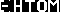
\includegraphics[width=3.5in]{q3o.png} 
	\caption{Recall with 30\% different data.   }\label{fig:1} 
\end{figure} 
\spar
From this experiment, we can see in this kind of memory, the recall accurancy only depends on the difference between the input and training set. It's independent of the similarty between the input and desired output.
\end{document}


